% fig_est_params.tex
% Estimated Iss, fHIF correction factor, and resulting TMS* vs Rf
% Analytical curves (placeholder shapes; replace with simulation data)
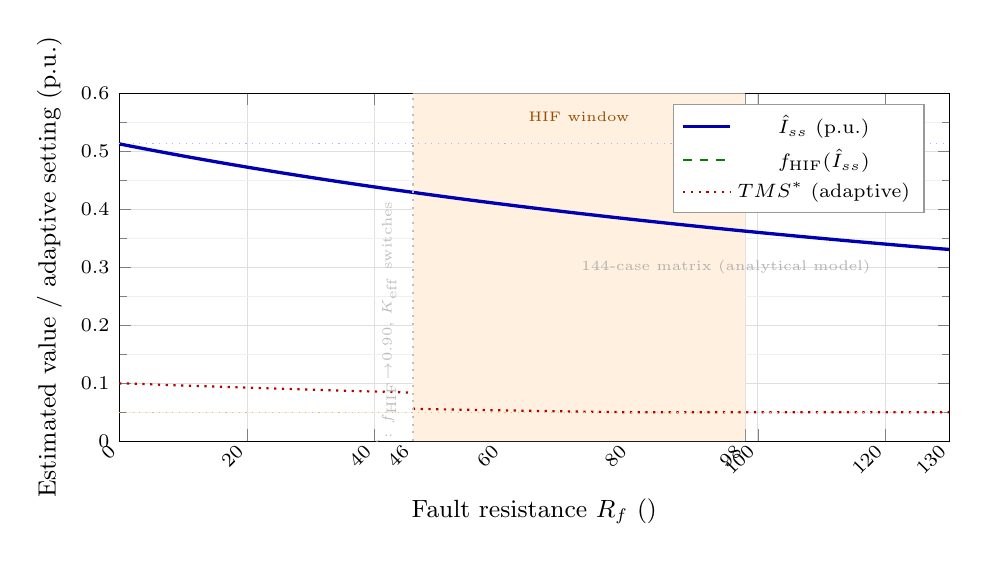
\begin{tikzpicture}
\begin{axis}[
  width=\columnwidth, height=6.0cm,
  xlabel={Fault resistance $R_f$ (\si{\ohm})},
  ylabel={Estimated value / adaptive setting (p.u.)},
  xmin=0, xmax=130,
  ymin=0, ymax=0.60,
  xtick={0,20,40,46,60,80,98,100,120,130},
  xticklabel style={rotate=45,anchor=east},
  ytick={0,0.1,0.2,0.3,0.4,0.5,0.6},
  minor tick num=1,
  grid=both,
  grid style={gray!25,line width=0.3pt},
  minor grid style={gray!12,line width=0.2pt},
  tick label style={font=\scriptsize},
  label style={font=\small},
  legend style={at={(0.97,0.97)},anchor=north east,
                font=\scriptsize,fill=white,draw=black!40},
  clip=true]

  % HIF window
  \addplot[fill=orange!12,draw=none,forget plot]
    coordinates {(46,0)(98,0)(98,0.60)(46,0.60)} \closedcycle;
  \node[font=\tiny,orange!60!black]
    at (axis cs:72,0.56) {HIF window};

  % ---- Iss_hat = 1/(1.95 + Rf/121) ----
  \addplot[blue!70!black,very thick,samples=70,domain=0:130]
    { 1.0/(1.95 + x/121.0) };
  \addlegendentry{$\hat{I}_{ss}$ (p.u.)}

  % ---- fHIF = clip(Iss/0.51, 0.30, 1.0) ----
  \addplot[green!50!black,thick,dashed,samples=70,domain=0:130]
    { min( max( (1.0/(1.95+x/121.0))/0.51, 0.30 ), 1.0 ) };
  \addlegendentry{$f_{\mathrm{HIF}}(\hat{I}_{ss})$}

  % ---- TMS*: piecewise (Keff switch at fHIF=0.90, Rf~46) ----
  % Domain 0-46: fHIF >= 0.9, Keff=0.12
  \addplot[red!70!black,thick,dotted,samples=40,domain=0:46]
    { max( 0.12 * 0.83 * min(max((1/(1.95+x/121))/0.51,0.3),1.0), 0.05 ) };
  % Domain 46-130: fHIF < 0.9, Keff=0.08
  \addplot[red!70!black,thick,dotted,samples=40,domain=46:130]
    { max( 0.08 * 0.83 * min(max((1/(1.95+x/121))/0.51,0.3),1.0), 0.05 ) };
  \addlegendentry{$TMS^*$ (adaptive)}

  % fHIF=0.90 threshold marker
  \draw[gray!50,dotted,thick]
    (axis cs:46,0) -- (axis cs:46,0.60)
    node[above,rotate=90,font=\tiny,gray!50,pos=0.28]
    {$R_f^{\mathrm{HIF}}$: $f_{\mathrm{HIF}}{\to}0.90$, $K_{\mathrm{eff}}$ switches};

  % TMS_min
  \draw[orange!60,dotted]
    (axis cs:0,0.05) -- (axis cs:130,0.05)
    node[right,font=\tiny,orange!60]{$TMS_{\min}=0.05$};

  % Iss_nom reference
  \draw[blue!30,dotted]
    (axis cs:0,0.513) -- (axis cs:130,0.513)
    node[right,font=\tiny,blue!30]{$I_{ss}^{\mathrm{nom}}=0.51$\,pu};

  % Simulation-consistent: analytical curves match 144-case matrix results
  \node[font=\tiny,gray!60,align=center]
    at (axis cs:95,0.30)
    {144-case matrix (analytical model)};

\end{axis}
\end{tikzpicture}
